\documentclass[10pt,letterpaper]{article}

\usepackage[margin=0.75in]{geometry}
\usepackage{graphicx}
\usepackage{booktabs}
\usepackage{array}
\usepackage{tabularx}
\usepackage{hyperref}
\usepackage{xcolor}
\usepackage{enumitem}
\usepackage{caption}
\usepackage{subcaption}
\usepackage{float}

\hypersetup{
  colorlinks=true,
  linkcolor=blue!50!black,
  citecolor=blue!50!black,
  urlcolor=blue!50!black
}

\setlist[itemize]{leftmargin=1.25em, itemsep=0.2em, topsep=0.25em}
\setlength{\parskip}{0.45em}
\setlength{\parindent}{0pt}

\title{\vspace{-1.5em}Benchmarking Robot Memory Under Interference\\
\large A Cross-Session Benchmark for Memory-Augmented VLAs}
\author{Soumil Shah}
\date{}

\begin{document}
\maketitle

\begin{abstract}
Modern robot policies increasingly use memory mechanisms to condition action on prior visual experience. Most evaluations focus on short or within-episode histories. Real deployed robots instead accumulate many unrelated experiences between the session where useful information is observed and the session where it is needed. We introduce RoboMME-Interference, a cross-session interference protocol over RoboMME task families that composes query episodes with relevant prior lessons and varying numbers of unrelated distractor sessions. We evaluate nine runnable memory-policy variants across nine task families and 18,450 rollouts. Perceptual memory systems, especially FrameSamp-Modul, substantially improve success when relevant history is nearby, while performance decays as distractor sessions push that history farther back. The benchmark exposes a practical failure mode for robot memory systems: systems must preserve helpful memory under realistic cross-session interference.
\end{abstract}

\section{Introduction}

Robots deployed in homes, warehouses, labs, or factories will accumulate experience across many sessions. They will see many users, many tasks, and many unrelated situations. A memory system that works only when the relevant information is nearby is fragile in realistic deployment histories.

The core question in this paper is simple: when a useful prior robot session is mixed into a longer history with unrelated sessions, do current robot memory systems still use it?

Our contribution is RoboMME-Interference, a cross-session interference protocol for RoboMME-style memory evaluation. For each query episode, we build a memory history from a relevant lesson session plus zero or more different-family distractor sessions. We then evaluate the same policy interface under \texttt{no-history}, \texttt{k0}, \texttt{k1}, \texttt{k3}, and \texttt{k7}. This turns memory distance and interference into measurable quantities.

Main findings:
\begin{itemize}
  \item Perceptual memory systems show strong near-session gains.
  \item FrameSamp-Modul is the strongest system in the current grid.
  \item TokenDrop-Modul is also strongly positive and lower than FrameSamp-Modul.
  \item The benefit decays as distractor sessions increase.
  \item Recurrent TTT variants are mostly flat in this setting.
\end{itemize}

\section{Related Work}

This section should position the paper against three clusters of work:
\begin{itemize}
  \item Vision-language-action policies, especially pi0.5-style robot policies that map visual observations and language instructions to action.
  \item Robot memory benchmarks such as RoboMME, which evaluate memory-augmented robot policies and primarily focus on memory available within a task or short context.
  \item Long-context and memory systems, including frame sampling, token dropping, recurrent memory, retrieval, and context compression.
\end{itemize}

The gap we target is cross-session interference. The core measurement is whether memory survives when unrelated robot experience is inserted between the relevant session and the query.

\section{RoboMME-Interference Protocol}

\begin{figure}[H]
  \centering
  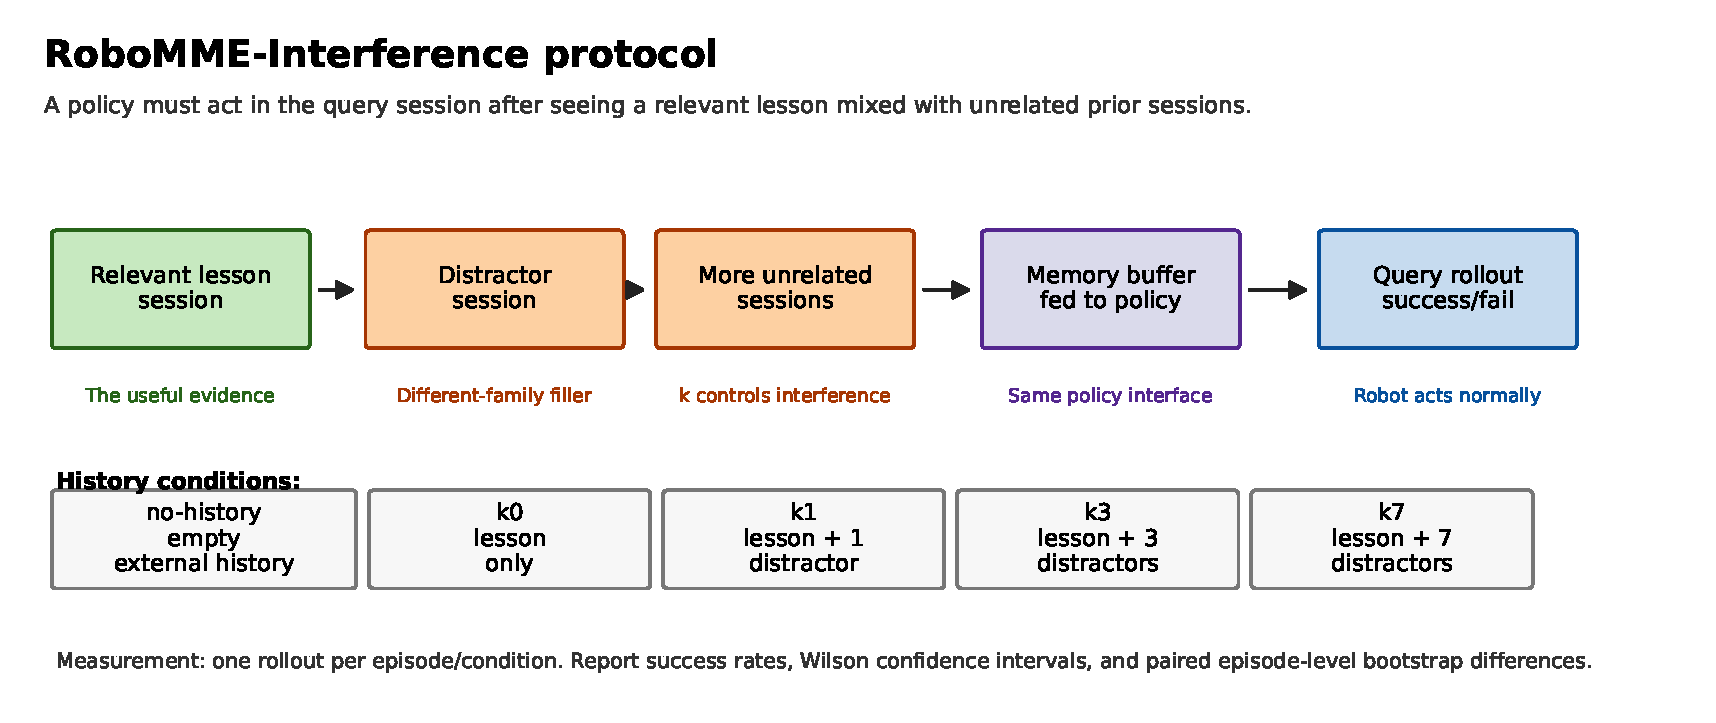
\includegraphics[width=\linewidth]{figures/protocol_diagram.pdf}
  \caption{RoboMME-Interference protocol. Each query episode is evaluated with an external history buffer. In \texttt{no-history}, the external history is empty. In \texttt{k0}, the history contains only the relevant lesson session. In \texttt{k1}, \texttt{k3}, and \texttt{k7}, the relevant lesson is followed by one, three, or seven unrelated different-family distractor sessions. The policy interface is unchanged; only the history buffer changes.}
  \label{fig:protocol}
\end{figure}

We evaluate nine structural RoboMME task families: MoveCube, RouteStick, VideoUnmask, VideoUnmaskSwap, VideoRepick, VideoPlaceButton, VideoPlaceOrder, InsertPeg, and PatternLock.

Each task family contributes 50 test episodes. Each memory system is evaluated on the same episode identities under the same history conditions. This gives paired comparisons between conditions, which is why the analysis reports both Wilson confidence intervals for individual success rates and paired episode-level bootstrap intervals for condition differences.

The key protocol choice is that distractor sessions come from different task families. This avoids constructing arbitrary wrong-prior facts inside the same task family. The benchmark is therefore measuring interference from unrelated robot experience, which is the deployment-like failure mode we care about.

\section{Memory Systems}

We evaluate nine runnable systems:
\begin{itemize}
  \item Baseline: pi0.5 baseline.
  \item Perceptual memory systems: FrameSamp-Modul, TokenDrop-Modul, FrameSamp-Context, FrameSamp-Expert, TokenDrop-Context, and TokenDrop-Expert.
  \item Recurrent memory systems: Recurrent-TTT-Expert and Recurrent-TTT-Context.
\end{itemize}

The headline grid excludes symbolic or oracle-style systems. Those systems rely on privileged or structured information rather than the same visual-history pathway, so they fit better as ceilings or implementation notes.

\section{Experiments}

The final grid contains nine task families, nine memory systems, five history conditions, 50 test episodes per family, 18,450 completed rollouts, and 369 / 369 complete result cells.

Primary result sources:
\begin{itemize}
  \item \texttt{tables/main\_success\_rates.csv}
  \item \texttt{tables/family\_success\_rates.csv}
  \item \texttt{tables/paired\_bootstrap\_comparisons.csv}
  \item \texttt{tables/result\_manifest.json}
\end{itemize}

Statistical treatment:
\begin{itemize}
  \item Individual success rates use Wilson 95\% confidence intervals.
  \item Within-system comparisons use paired episode-level bootstrap confidence intervals, because the same episode identities appear across history conditions.
\end{itemize}

\begin{table}[H]
  \centering
  \small
  \begin{tabularx}{\linewidth}{lccccc}
    \toprule
    System & No history & k0 & k1 & k3 & k7 \\
    \midrule
    pi0.5 baseline & 17.3\% & -- & -- & -- & -- \\
    FrameSamp-Modul & 18.2\% & 45.3\% & 38.4\% & 30.0\% & 19.3\% \\
    TokenDrop-Modul & 17.1\% & 35.3\% & 30.9\% & 23.6\% & 19.8\% \\
    FrameSamp-Context & 17.8\% & 26.7\% & 18.7\% & 18.7\% & 17.8\% \\
    FrameSamp-Expert & 17.6\% & 27.1\% & 20.9\% & 19.6\% & 19.6\% \\
    TokenDrop-Context & 13.8\% & 22.9\% & 19.1\% & 15.3\% & 13.1\% \\
    TokenDrop-Expert & 16.9\% & 27.3\% & 20.2\% & 15.6\% & 14.0\% \\
    Recurrent-TTT-Expert & 16.0\% & 18.0\% & 16.4\% & 16.2\% & 15.6\% \\
    Recurrent-TTT-Context & 16.9\% & 15.3\% & 16.2\% & 17.6\% & 14.0\% \\
    \bottomrule
  \end{tabularx}
  \caption{Main success rates across all nine task families. The full table with Wilson 95\% confidence intervals is in \texttt{tables/main\_success\_rates.csv}.}
  \label{tab:main-success}
\end{table}

\section{Results}

\subsection{Overall Cross-Session Performance}

\begin{figure}[H]
  \centering
  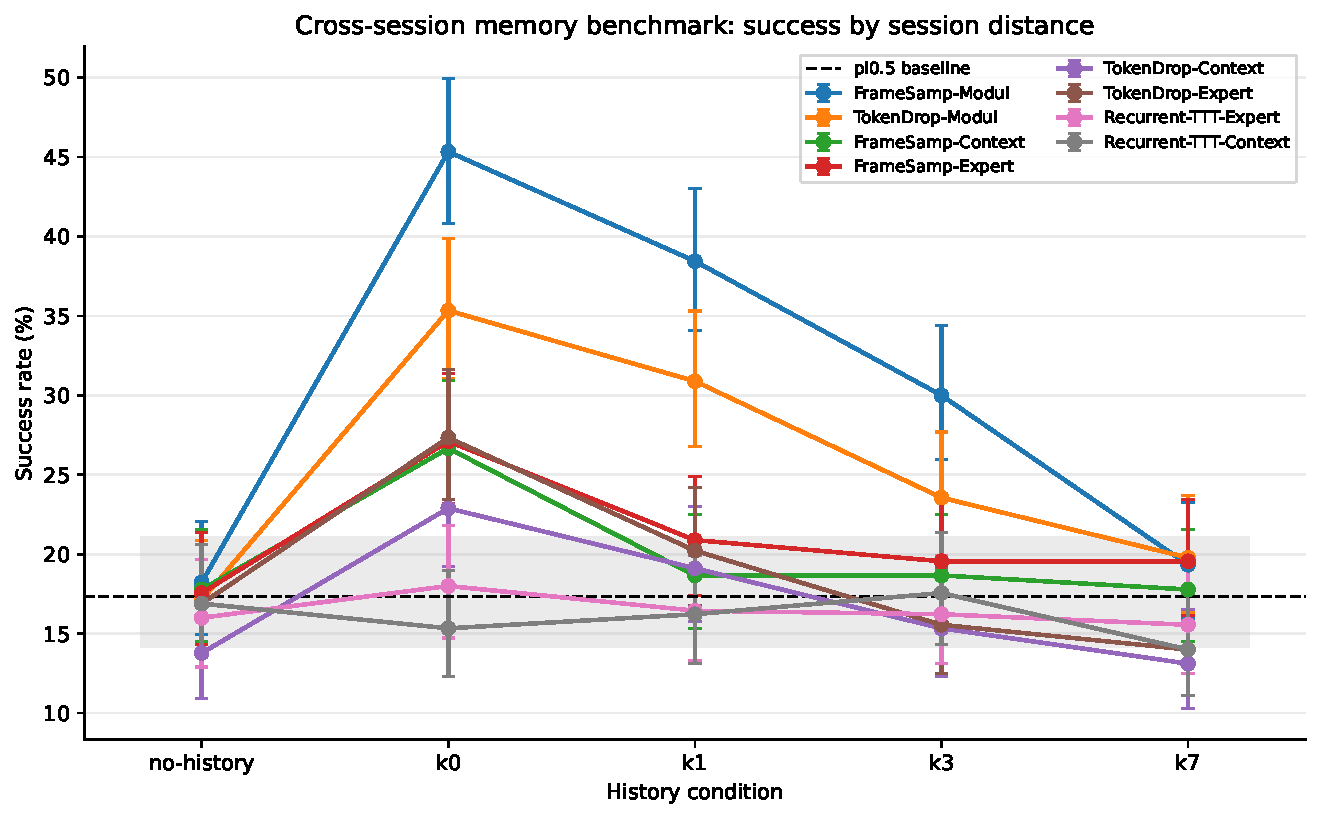
\includegraphics[width=\linewidth]{figures/overall_plain_success_by_condition.pdf}
  \caption{Overall success rate by memory system and history condition across all nine task families. The dashed line is the pi0.5 baseline. Perceptual memory systems improve substantially when the relevant lesson is nearby, especially FrameSamp-Modul and TokenDrop-Modul. As distractor sessions increase, success decays toward the no-history floor.}
  \label{fig:overall}
\end{figure}

Headline numbers:
\begin{itemize}
  \item FrameSamp-Modul: 18.2\% no-history, 45.3\% k0, 38.4\% k1, 30.0\% k3, 19.3\% k7.
  \item TokenDrop-Modul: 17.1\% no-history, 35.3\% k0, 30.9\% k1, 23.6\% k3, 19.8\% k7.
  \item pi0.5 baseline: 17.3\%.
  \item Recurrent TTT variants remain close to baseline across conditions.
\end{itemize}

Interpretation:
\begin{itemize}
  \item Visual memory can help substantially.
  \item Each memory system has its own no-history condition, so the curve isolates history use rather than checkpoint strength alone.
  \item The important shape is the curve: near-session memory helps; longer cross-session interference erodes the benefit.
\end{itemize}

\subsection{Interference Sensitivity}

\begin{figure}[H]
  \centering
  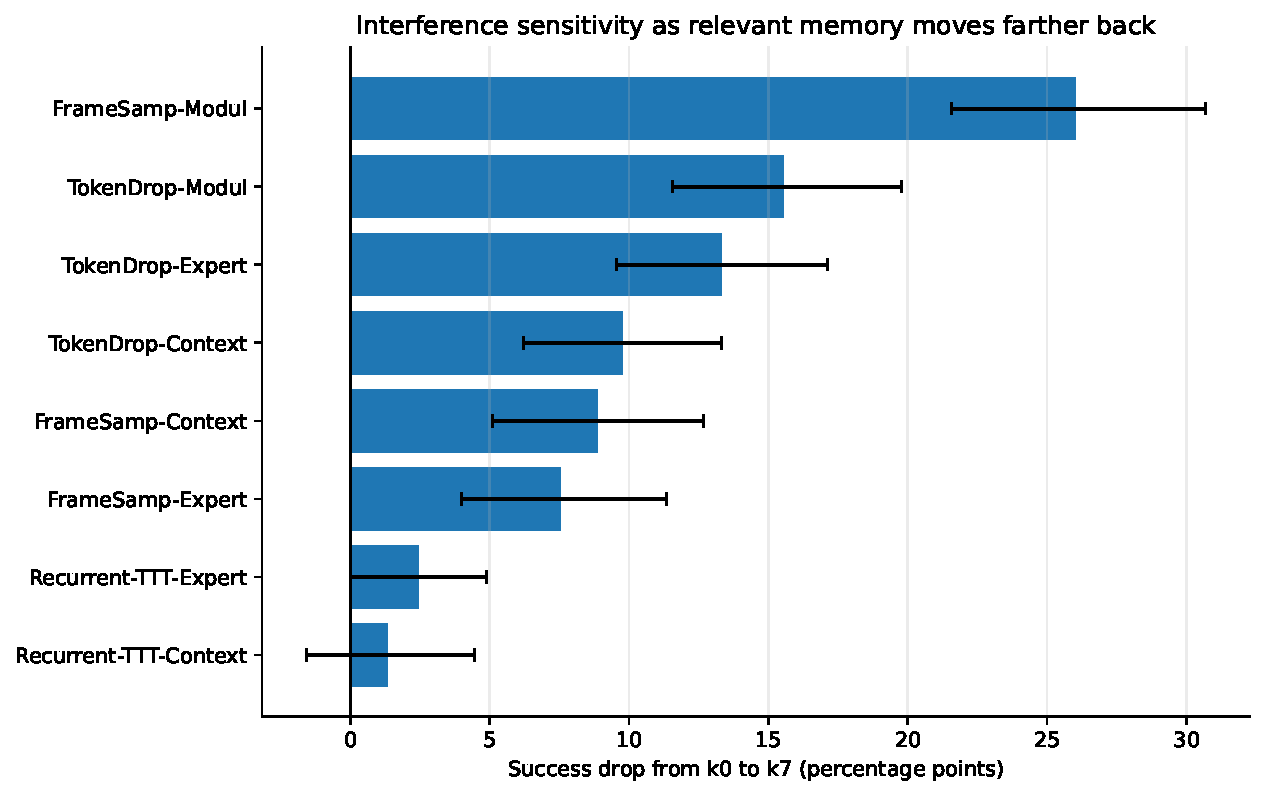
\includegraphics[width=0.82\linewidth]{figures/interference_drop_k0_to_k7.pdf}
  \caption{Success drop from \texttt{k0} to \texttt{k7}, measured with paired episode-level bootstrap intervals. Systems with strong near-history gains also show measurable degradation when the relevant lesson is pushed behind seven distractor sessions. This is the benchmark's main interference signal.}
  \label{fig:interference}
\end{figure}

Key effects:
\begin{itemize}
  \item FrameSamp-Modul gains 27.1 percentage points at \texttt{k0} over no-history, with bootstrap CI 22.7 to 31.6 percentage points.
  \item TokenDrop-Modul gains 18.2 percentage points at \texttt{k0} over no-history, with bootstrap CI 14.0 to 22.4 percentage points.
  \item FrameSamp-Modul drops about 26.0 percentage points from \texttt{k0} to \texttt{k7}.
  \item TokenDrop-Modul drops about 15.6 percentage points from \texttt{k0} to \texttt{k7}.
\end{itemize}

Interpretation:
\begin{itemize}
  \item The benchmark measures both near-history benefit and long-history degradation.
  \item It measures how quickly the benefit collapses as irrelevant prior sessions accumulate.
\end{itemize}

\subsection{Per-Family Behavior}

\begin{figure}[H]
  \centering
  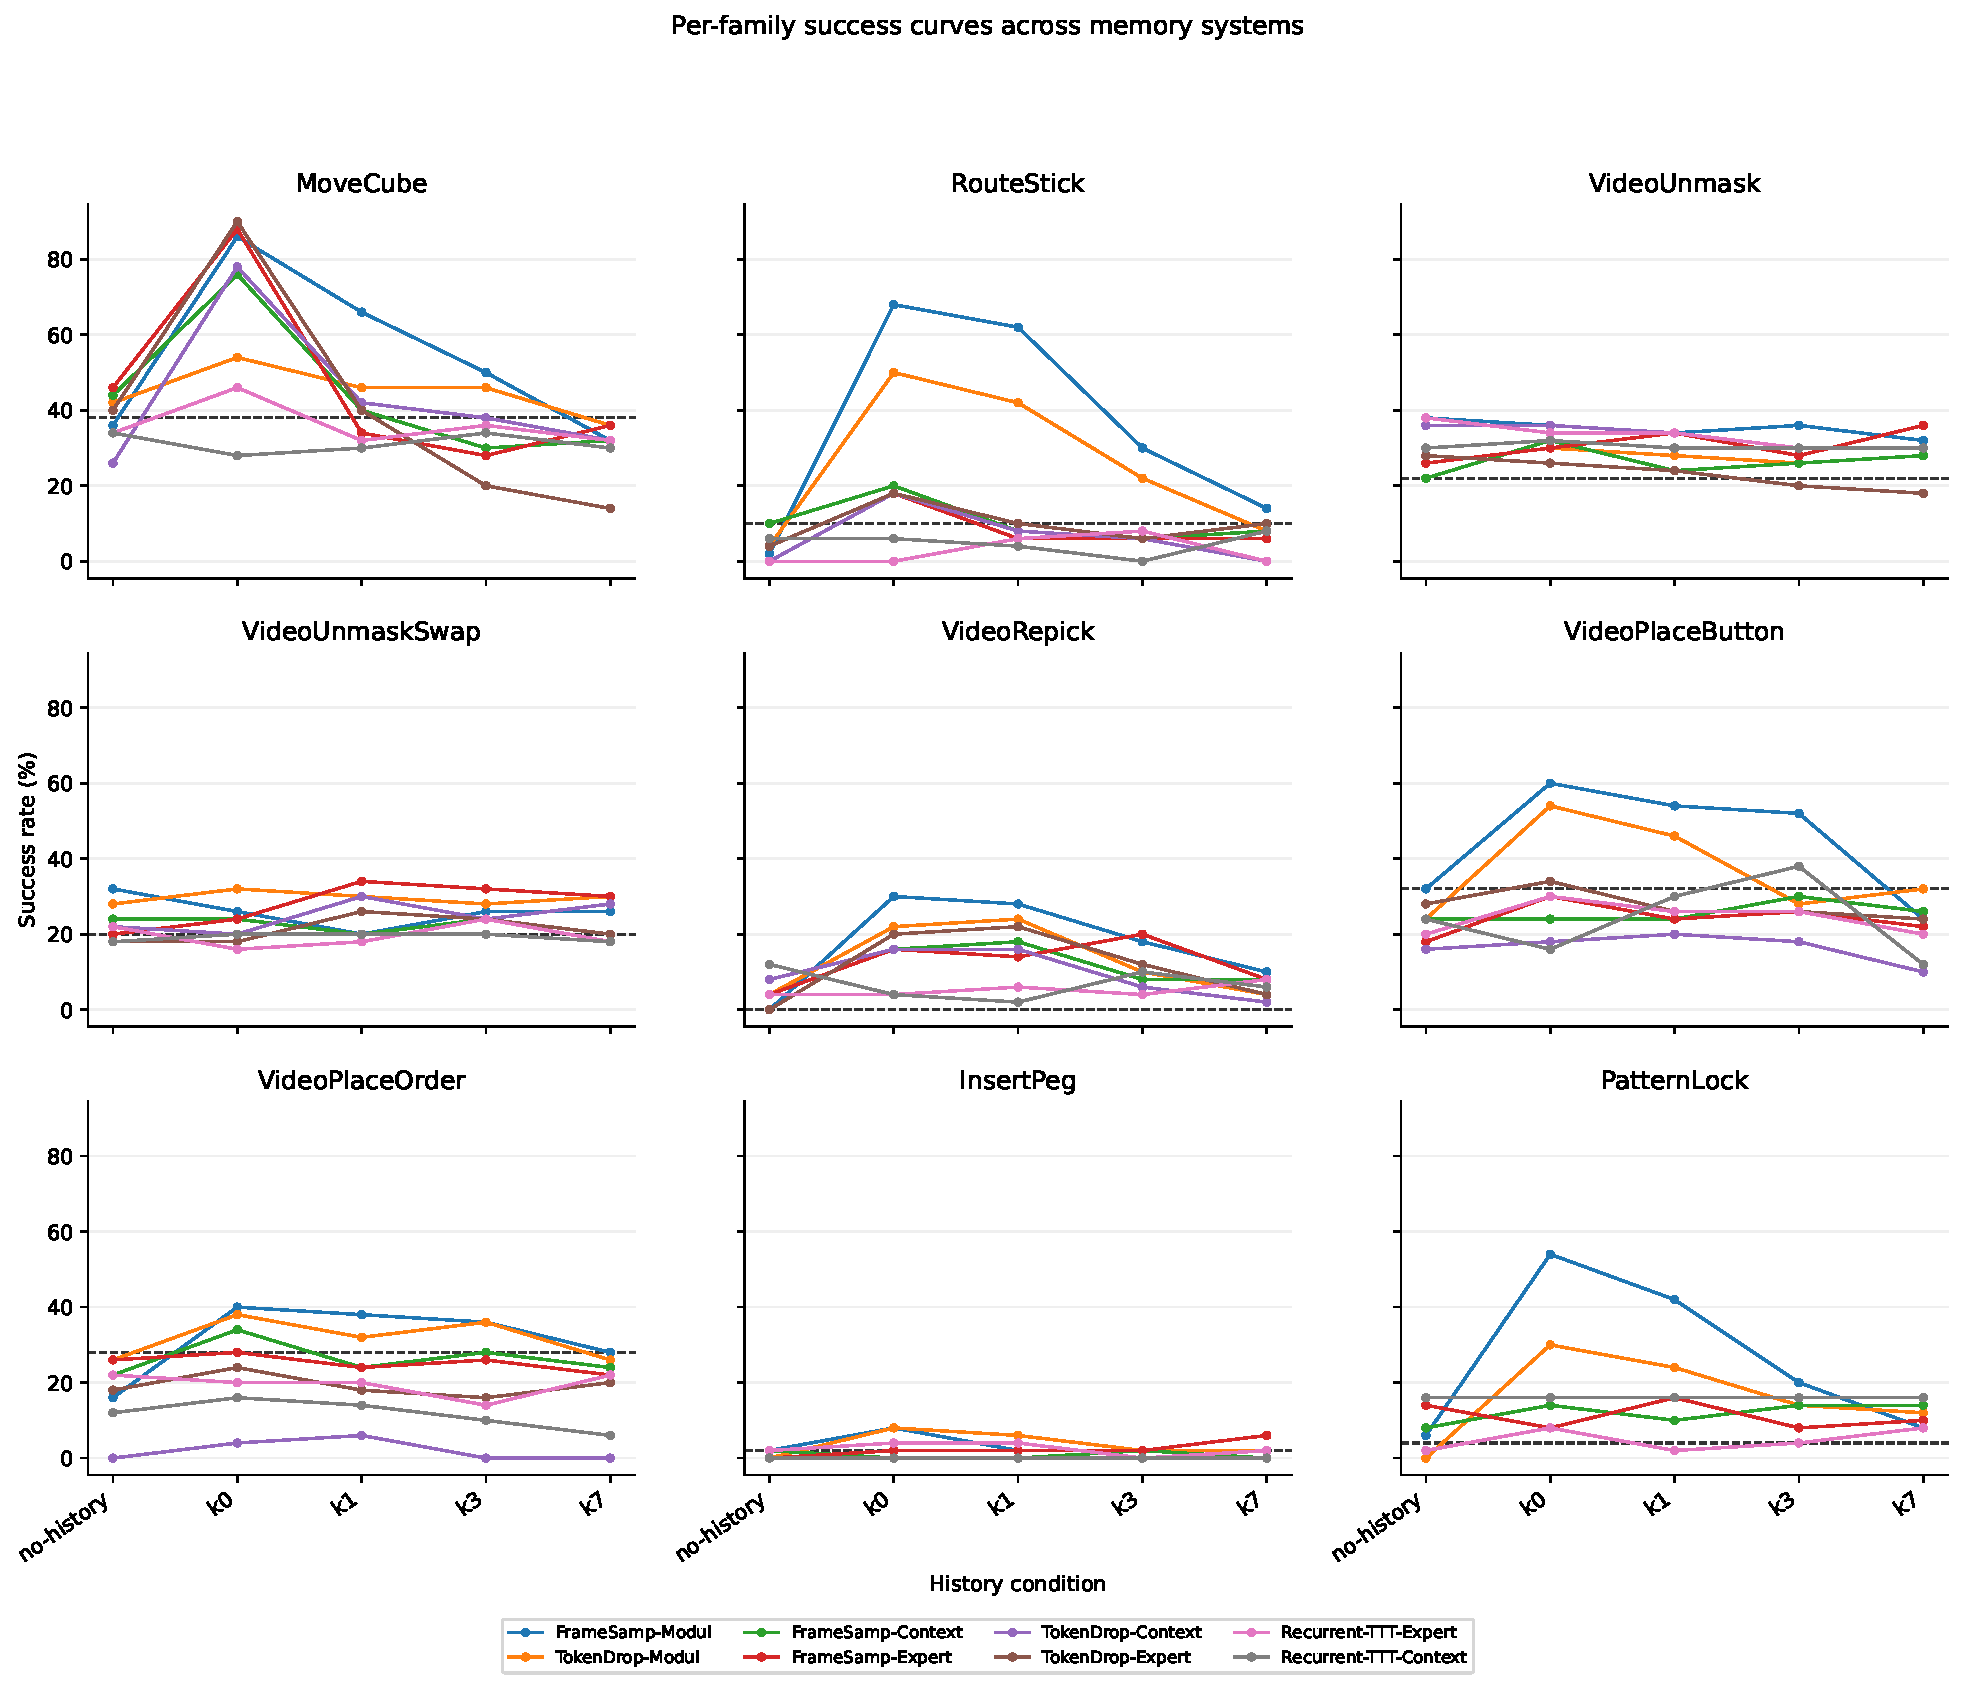
\includegraphics[width=\linewidth]{figures/per_family_plain_success_small_multiples.pdf}
  \caption{Per-family success curves for all evaluated memory systems. The aggregate result is not uniform: some families have high floors, some have low ceilings, and some show clear memory sensitivity. This motivates reporting both aggregate and per-family results.}
  \label{fig:family-curves}
\end{figure}

\begin{figure}[H]
  \centering
  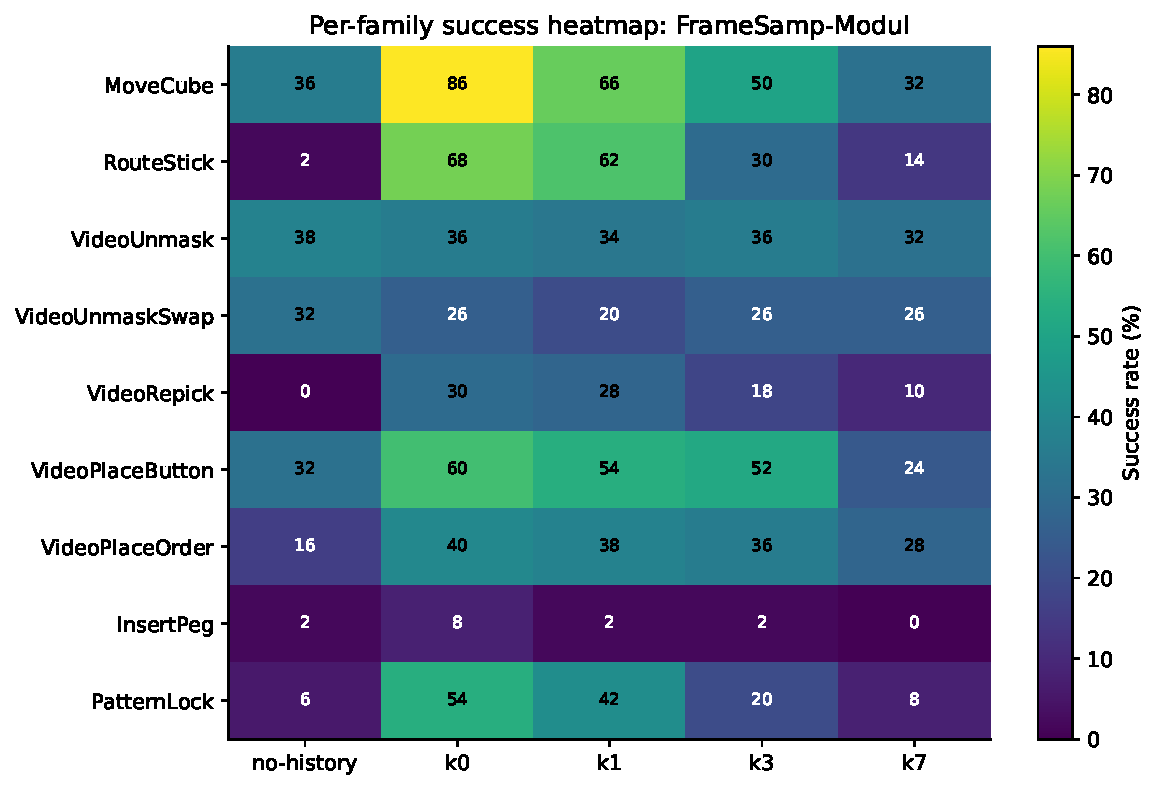
\includegraphics[width=0.72\linewidth]{figures/framesamp_modul_family_heatmap.pdf}
  \caption{Per-family heatmap for FrameSamp-Modul, the strongest overall variant. The heatmap shows where the near-session gain appears and where it survives or collapses as distractors are added.}
  \label{fig:framesamp-heatmap}
\end{figure}

Interpretation:
\begin{itemize}
  \item The benchmark should be presented with family-level results alongside aggregate scores.
  \item Some tasks are mostly competence-limited; others reveal memory sensitivity more clearly.
  \item The main paper can show the compact heatmap and move the dense all-variant small multiple to the appendix if space is tight.
\end{itemize}

\subsection{Difficulty Effects}

\begin{figure}[H]
  \centering
  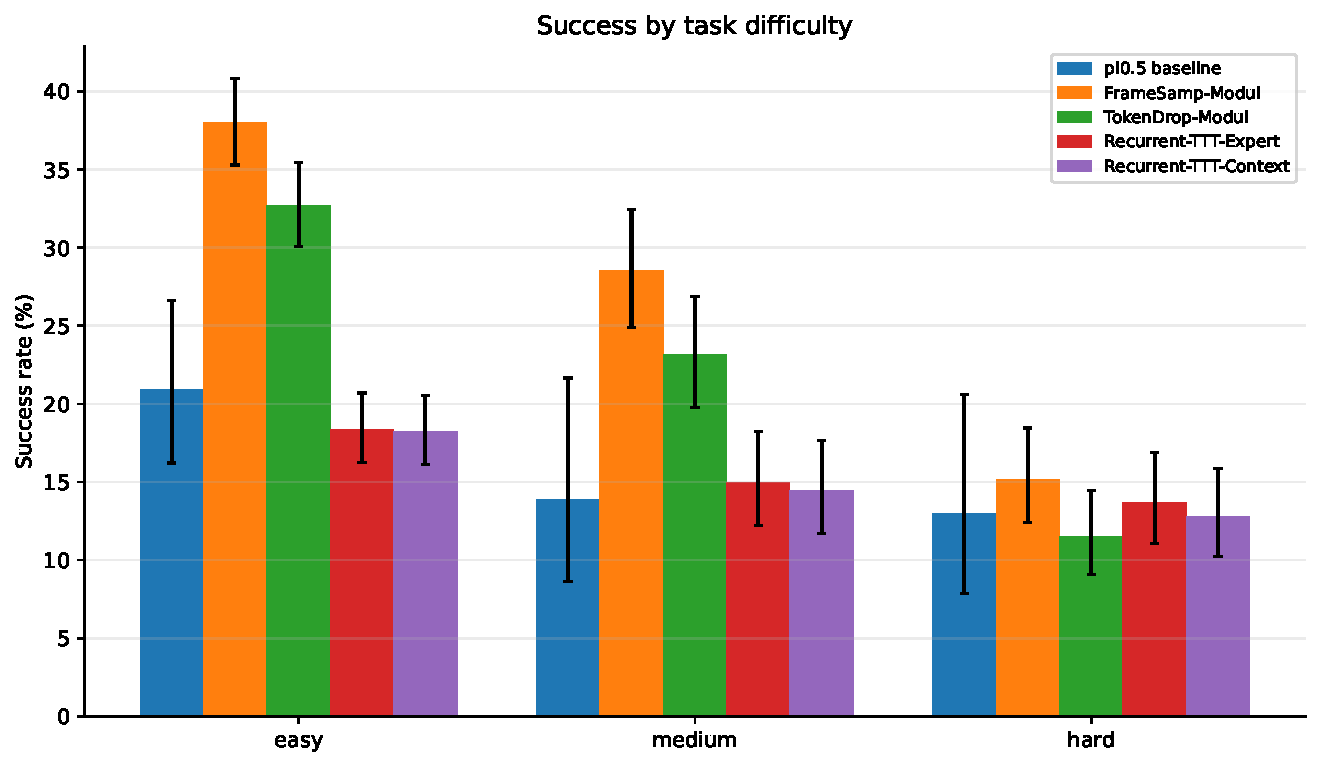
\includegraphics[width=0.86\linewidth]{figures/difficulty_plain_success.pdf}
  \caption{Success rates by task difficulty. Easy and medium episodes show clearer separation between systems, while hard episodes compress the spread because many systems fail. This helps explain why aggregate memory gains are not uniform across the full benchmark.}
  \label{fig:difficulty}
\end{figure}

Interpretation:
\begin{itemize}
  \item Difficulty is a confound that should be reported, not hidden.
  \item Hard cases are useful for completeness. The cleanest memory signal appears where the policy has enough base competence to act on memory.
\end{itemize}

\section{Discussion}

The main story is strong enough for a workshop-style benchmark paper: cross-session memory is measurably different from short-context memory, and the current systems behave differently under interference.

What the result says:
\begin{itemize}
  \item Perceptual memory is useful when the relevant session is near the query.
  \item Frame sampling appears more robust than token dropping in this setup.
  \item Recurrent variants remain mostly flat in the cross-session setting.
  \item A useful robot memory benchmark should report both memory benefit and interference sensitivity.
\end{itemize}

Scope boundaries:
\begin{itemize}
  \item FrameSamp-Modul is the strongest system in this evaluated grid.
  \item The benchmark is a measurement tool for robot memory under interference.
  \item Real-world evaluation remains necessary.
  \item The grid covers released runnable variants, not every retrieval or memory-writing architecture.
\end{itemize}

The public value is the benchmark itself: the protocol, the runnable result grid, and the analysis package give future memory systems a concrete target.

\section{Limitations}

Current limitations:
\begin{itemize}
  \item Simulator-only evaluation.
  \item Built on selected RoboMME structural task families.
  \item Evaluates released/runnable variants, not every possible memory architecture.
  \item Does not include per-step action traces in the current public result bundle.
  \item Some families have high no-history floors or low absolute success ceilings.
\end{itemize}

These are acceptable for a workshop artifact if they are stated cleanly and the release makes the protocol easy to extend.

\section{Conclusion}

Cross-session memory is a distinct robotics capability. A robot memory system must do more than use a helpful frame when it is nearby; it must preserve and select useful prior experience despite unrelated intervening sessions. Our benchmark makes that measurable. Across 18,450 rollouts, perceptual memory systems show strong near-session benefits and clear degradation under interference, while recurrent variants remain mostly flat. This gives the community a concrete benchmark target for long-horizon robot memory.

\appendix
\section{Supporting Analysis}

\begin{figure}[H]
  \centering
  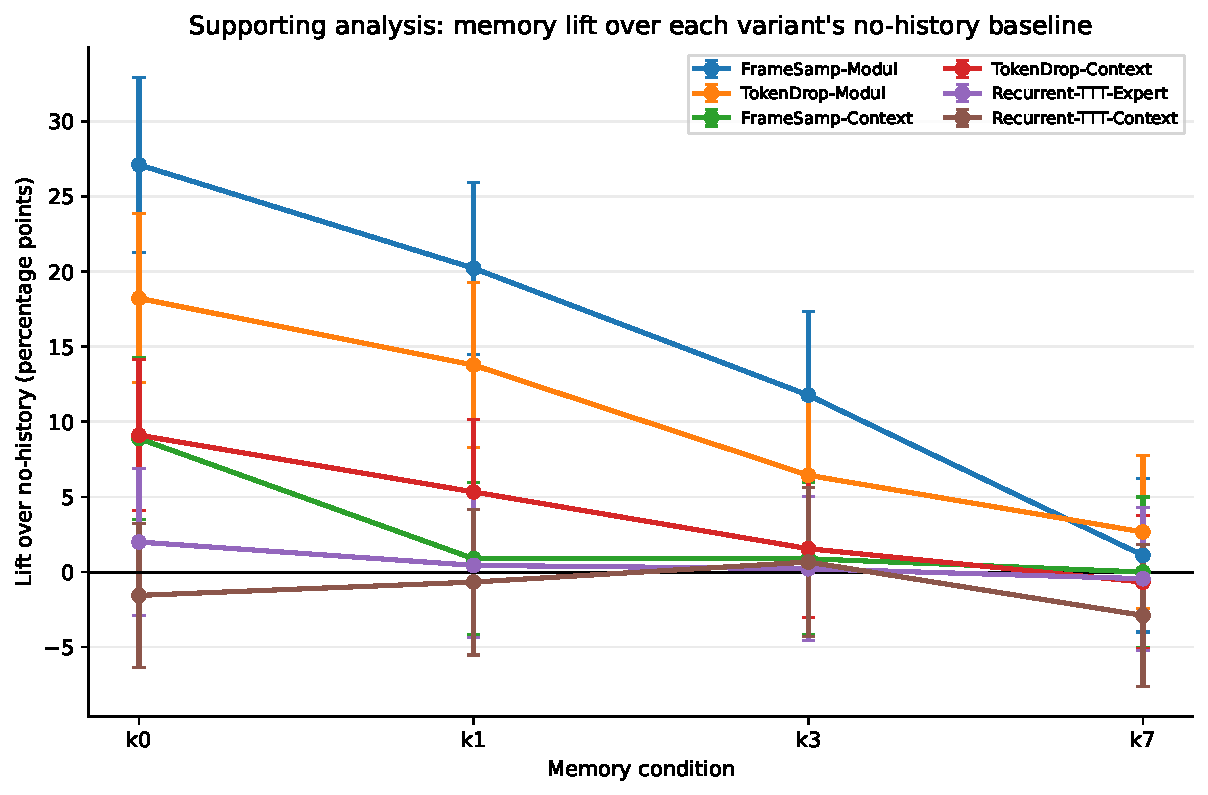
\includegraphics[width=0.9\linewidth]{figures/memory_lift_vs_no_history.pdf}
  \caption{Lift over each memory system's own no-history condition. This is supporting analysis; the main paper leads with plain success rates because no-history performance differs across checkpoints and memory-system implementations.}
\end{figure}

\begin{figure}[H]
  \centering
  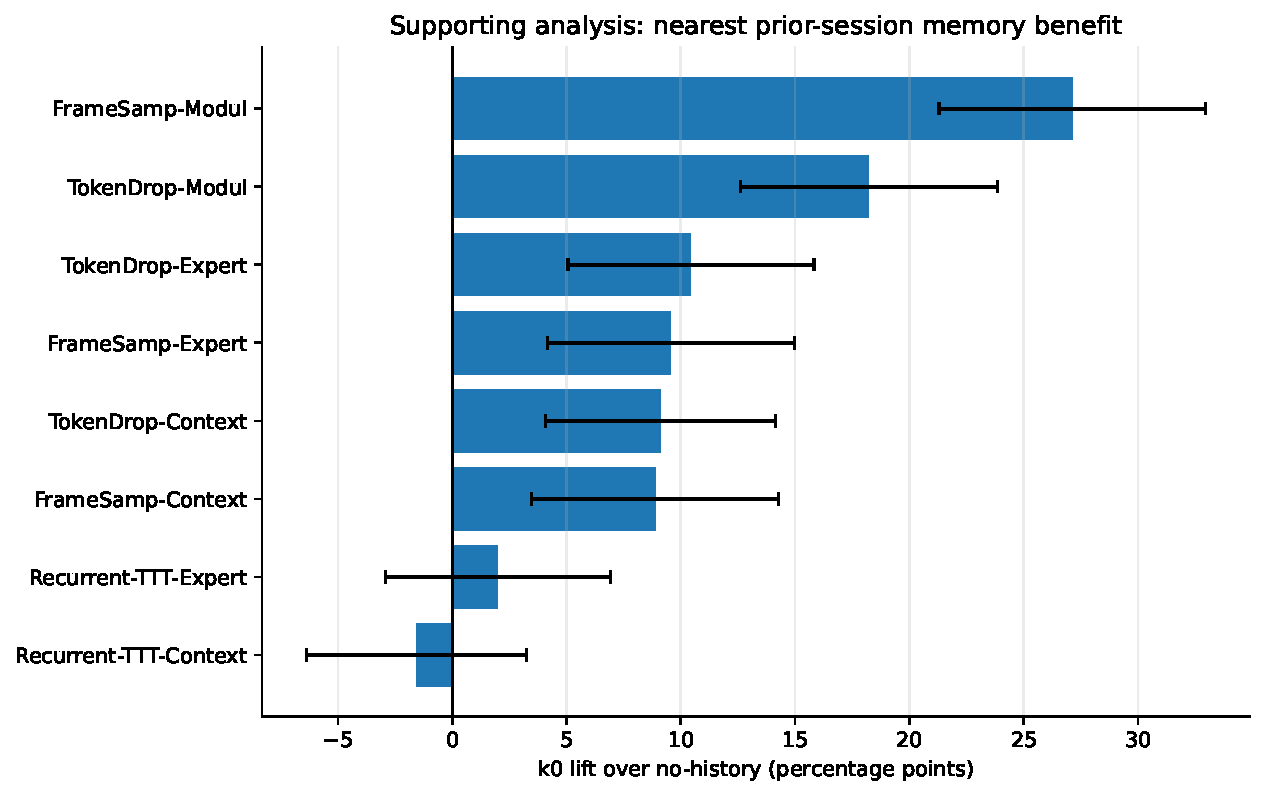
\includegraphics[width=0.78\linewidth]{figures/k0_lift_ranking.pdf}
  \caption{Nearest-prior lift ranking at \texttt{k0}. Perceptual memory variants dominate the positive improvements; recurrent variants are flat or weak.}
\end{figure}

\end{document}
